\documentclass[11pt,a4paper,openright]{report}
\usepackage[utf8]{inputenc}
\usepackage{graphicx}
\graphicspath{ {images/} }
\usepackage[czech]{babel}
\usepackage[top=25mm,bottom=25mm,right=25mm,left=30mm,head=12.5mm,foot=12.5mm]{geometry}
\usepackage{titlesec}
\usepackage{amsmath}
\usepackage{listings}
\usepackage{fancyhdr}

\usepackage[sorting=none,backend=bibtex]{biblatex}
\bibliography{biblio.bib}

\titleformat{\chapter}[block]{\bfseries\Huge}{}{0em}{}
\titleformat{\section}[hang]{\bfseries\Large}{}{1em}{\thesection\enspace}

\pagestyle{fancy}
\fancyhf{}
\fancyhead[R]{CheapCopter}
\fancyhead[L]{\thechapter. Kapitola}
\fancyfoot[C]{\textbf{\thepage}}
\fancypagestyle{plain}{%  the preset of fancyhdr
    \fancyhf{} % clear all header and footer fields
    \fancyfoot[C]{\textbf{\thepage}} % except the center
    \renewcommand{\headrulewidth}{0pt}
    \renewcommand{\footrulewidth}{0pt}}

\title{CheapCopter}

\author{Filip Roček}

\date{\today}

\renewcommand*\contentsname{Obsah}

\begin{document}

%%% Titulní strana práce a další povinné informační strany

%%% Titulní strana práce

\pagestyle{empty}
\pagenumbering{gobble}
\hypersetup{pageanchor=false}

\begin{center}
\LARGE
\textbf{GYMNASIUM JANA KEPLERA}\\
{\large Parléřova 2/118, 169 00 Praha 6}

\vspace{\stretch{3}}


\includegraphics[width=.3\textwidth]{img/logo}

\vspace{\stretch{3}}

{\Huge\bfseries\NazevPrace}

\vspace{8mm}
\mdseries{Maturitní práce}

\vspace{\stretch{8}}
\large
\begin{tabular}{rl}
Autor: & \AutorPrace \\
\noalign{\vspace{2mm}}
Třída: & \Trida\\
\noalign{\vspace{2mm}}
Školní rok: & 2023/2024\\
\noalign{\vspace{2mm}}
Předmět: & Informatika \\
\noalign{\vspace{2mm}}
Vedoucí práce: & \Vedouci \\
\end{tabular}

\vspace{20mm}
Praha, \DatumOdevzdani
\end{center}


\openright

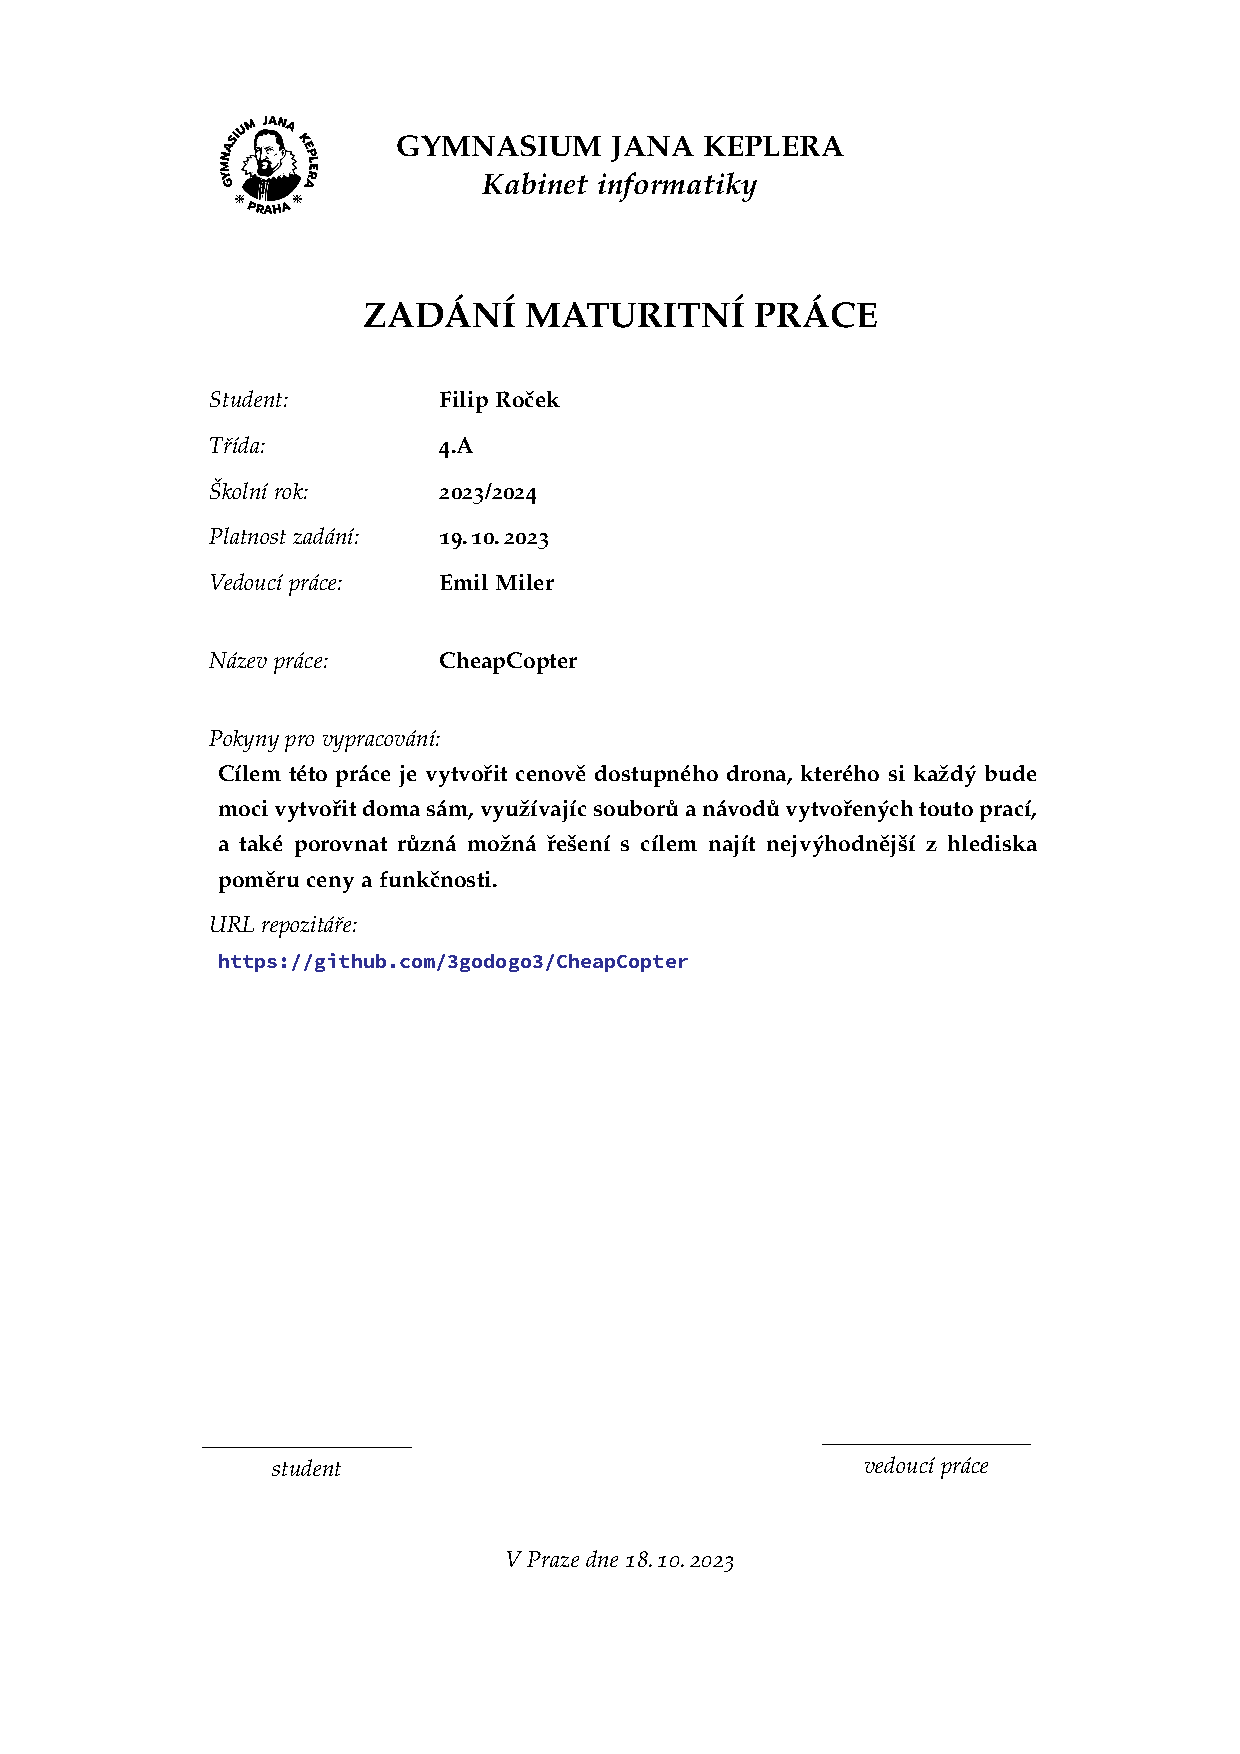
\includepdf[]{zadani.pdf}


%%% Strana s čestným prohlášením k bakalářské práci

\hypersetup{pageanchor=true}
\cleardoublepage
\vspace*{\fill}
\section*{Prohlášení}
\noindent
\Prohlaseni

\vspace{2cm}
\noindent
V Praze dne \today
\hspace*{\fill}\small{\AutorPrace}
\vspace{1cm}

%%% Povinná informační strana bakalářské práce
\openright
\section*{Abstrakt}
\noindent
\Abstrakt

\openright
\pagenumbering{arabic}

\clearpage
\thispagestyle{empty}

\vspace*{\fill}

Prohlašuji, že jsem tuto práci vypracoval samostatně a výhradně s použitím
citovaných pramenů, literatury a dalších odborných zdrojů.

\vspace{2mm}

Beru na vědomí, že se na moji práci vztahují práva a povinnosti vyplývající ze
zákona č. 121/2000 Sb., autorského zákona, v platném znění.

\vspace{15mm}

\begin{minipage}[t]{0.4\textwidth}
    \begin{flushleft}
        \emph{Dne:}\\
        \vspace{5mm}
        \rule[0.5em]{10em}{0.5pt}
    \end{flushleft}
\end{minipage}
\begin{minipage}[t]{0.5\textwidth}
    \begin{flushright}
        \emph{Podpis:} \\
        \vspace{5mm}
        \rule[0.5em]{10em}{0.5pt}
    \end{flushright}
\end{minipage}

\vspace{10mm}


\tableofcontents

\chapter{Abstrakt}
Tato práce shrnuje tvorbu vlastního drona, kterého si kdokoliv se základními znalostmi pájení, dokáže doma vyrobit.

První část se zaobírá volbou vhodných komponent pro funkčnost tohoto projektu a jejich využitím.

Druhá kapitola rozebírá tvorbu a úpravou vlastního tištěného spoje, který propojuje všechny komponenty drona.

Třetí oddíl pojednává o součástích tvořených s pomocí 3D tiskárny, ucelujících celý projekt.

Poslední část řeší skutečné použití a fungčnost vytvořeného drona.

\chapter{Výběr součástek}
\section{Ovládání}

\subsection*{Procesor}
    Pro samotné fungování a ovládání drona je potřeba procesor, který bude vzdáleně přijímat příkazy a předávat je jednotlivým částem drona. Pro tento úkol jsem zvolil čim ESP-WROOM32 pro jeho nízkou hmotnost, implementovanou podporu Wi-Fi a jeho dvě jádra, která umožňují pruběh více procesů zároveň.
    
\subsection*{Gyroskop}
    Pro automatické vyvažování drona musíme přidat také gyroskop, protože bouhužel námi vyraný procesor jej neobsahuje. Pro projekt nám bude vyhovovat tří-osý gyroskop s akcelerometrem MPU-6050. Tato komponenta je schopna změřit odchylku na třech hlavních osách, podle které upravíme rychlost motorů pro vyrovnání drona. Změřené odchylky si nazveme "ROLL" pro osu x, "PITCH" pro osu y a "YAW" pro osu z.
    
\section{Pohon}

\subsection*{Motory}
    Aby dron byl schopen letu, potřebujeme motory. Nejčastějším provedením je kvadrokoptéra, která má motory čtyři. Vybral jsem motory od BetaFPV, pro jejich nevelkou hmotnost, nízkou cenu a jejich časté použití v levných a lehkých dronech.\cite{motorv1} Výběr byl proveden po konzultaci s poradcem v obchodě FYFT.CZ, který mě obeznámil, že vypočítat přesně kolik motor je schopen unést a předem vědět, který motor vybrat nelze, je to pouze o dobrém odhadu a zkušenostech. Pro správné fungování je potřeba, aby se dva motory na diagonále otáčely stejným směrem a zbylé dva směrem opačným, čímž dosáhneme vynulování otáčení po ose z. Pokud by se všechny motory otáčely stejným směrem, dron by nám rotoval.
    
\newpage

\subsection*{L293D}
    Pro ovládání motoru využívám dva drivery L293D, kde každý ovládá dva motory. Tento driver funguje na principu dvou AND hradel, kde jedno je stále na hodnotě LOW a druhé má na vstupu hodnotu HIGH a PWM signál poskytnutý ESP. PWM signálem jsme schopni omezit rychlost otáček a snížit tím rychlost stoupání.
    
\section{Napájení}

\subsection*{Baterie}
    Nejvhodnější baterií pro takovýto projekt je typ Li-Pol, protože jsou lehké, s velkou kapacitou a mohou se nabíjet narozdíl od jiných baterií. S limitním napětím našich motorů hodnoceným na 5V potřebujeme dvojčlánkovou Li-Pol baterii s napětím 7,4V, které pomocí součástek v další části snížíme na požadovaných 5V. Po spočítání spotřeby motorů a čipů jsme se rozhodl pro baterii KAVAN Li-Po 860mAh/7,4V, která by měla vydržet při nejvyšší zátěži přibližně patnáct minut.
    
\subsection*{Regulace}
    Náš dron potřebuje dvě napětí - 3,3V pro ESP a MPU a 5V pro L293D a motory. V prvním provedení jsem tohoto dosáhl za pomocí dvou lineárních regulátorů napětí LM7805C zapojených do serie. Tento postup bohužel prakticky nefungoval, i když jsme dosáhli požadovaných napětí, první regulátor se ihned přehřál na kritickou teplotu a vypínal se. Řešením bylo vyměnit první regulátor z 7,4V na 5V za Step-Down converter, který je sice větší a těžší, ale efektivnější a nepřehřívá se.
    
    \begin{figure}[h]
        \centering
        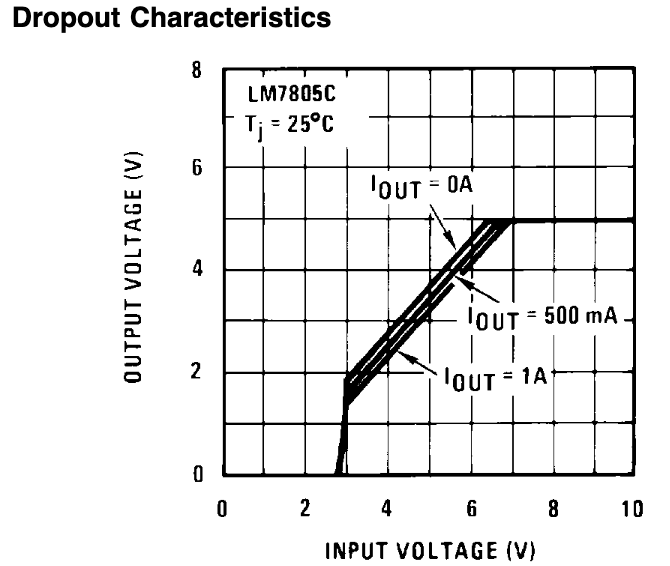
\includegraphics[scale=0.7]{images/regulartor.png}
        \caption{Výstupní napětí v závislosti na vstupním u regulátoru LM7805C\cite{LM7805C}}
    \end{figure}




\chapter{Tištěný spoj}
\section{Design}
    Tvorba PCB začala schématem zapojení všech komponent. K tomuto úkolu jsem využil software KiCad, který je velmi intuitivní i pro úplné začátečníky. Dále je potřeba navrhnout samotné PCB. Pro náš projekt bude dostatečné nejlevnější řešení PCB a to pevné dvouvrstvé bez zlatých pinů. Po doporučení vedoucího práce byl přidán GND do celé plochy tištěného spoje, kde se nevyskytují jiné propoje, pro jednoduché propojení všechs komponent. 

\section{Objednání}
    Pro samotné vytvoření tohoto tištěného spoje jsem si vybral stránku JLCPCB.COM, která umožňuje za velmi nízkou cenu(cca 100 Kč za pět kusů PCB), nechat si vyrobit jakékoliv PCB. Jediná nevýhoda je lokace společnosti. Sídlí v Číně, a proto doprava trvala tři týdny. Byla možnost si připlatit za doručení do několika dnů, ale částka by se vyšplhala i na 1000 Kč za samotnou dopravu, což je skoro vyšší částka než hodnota samotného dronu.


\chapter{Tělo drona}
\section{Rám}
    Pro správnou funkčnost drona je zapotřebí správný poměr pevnosti a hmotnosti těla. Tohoto jsem dosáhl odhadem, kde první verze měla plné dno, čímž byla konstrukce rámu značně pevnější, ale o několik desítek gramů těžžší. V druhé verzi jsem ztenčil všechny stěny, ubral materiál dna a přidal nožicky pod jednotlivé motory pro lepší ochranu drátů motorů. Tímto se sice snížila pevnost, ale díky robustnosti samotného PCB to není znát, a zároveň se snížila hmotnost. Jako poslední jsem se rozhodl využít materiál PLA, se kterým se jednodušeji tiskne a je levnější, protože vyšší pevnost jiných materiálů jako například ABS mi nepřipadala nutná. Veškerá tvorba modelů byla provedena v programu Autodesk Fusion 360 a Prusa Slicer.

\section{Vrtule}
    Při první verzi modelu jsem se pokusil vymodelovat a vytisknout i vrtule, ale po dlouhé snaze, se mi nedařilo vytvořit ideální tvar. Z toho důvodu jsem využil model z internetu. Po jeho vytisknutí a testování jsem se ale dostal k závěru, že s mně dostupným materiálem jsou vrtule příliš tvrdé a křehké, a proto jsem se uchýlil ke koupi 2" vrtulí. Tyto vrtule jsem vybral po konzultaci s poradcem z FYFT.CZ.

\chapter{Použití}
V této kapitole si popíšeme jak dron ovládat a zdali opravdu funguje.

\section{Připojení se}
    Po zapojení baterie se dron automaticky zapne. Několik vteřin na to se vytvoří Wi-Fi access point, který se základně jmenuje "Drone" a lze se k němu připojit za pomocí hesla "password". Jak jméno, tak heslo pro AP se dá změnit v kódu přepsáním proměnných *ssid a *password. Návod na nahrání upraveného kódu se podívejte do kapitoly 4.3. Pokud dron chcete ovládat, je zapotřebí se na tento AP připojit. Veškeré ovládání poté najdete ve vašem webovém prohlížeci na  adrese "192.168.4.1". K ovládání doporučuji používat mobilního telefonu, ale je možné využít i počítače.

\section{Ovládání}
    Na webové stránce vidíte jednoduché GUI, s devíti tlačítky - osm na samotné ovládání drona a jedno na updatování firmware. Pro zapnutí motorů drona zmáčkněte tlačítko "ON". Dále pro vzlédnutí využijte levého dolního tlačítka "UP" a pro pokles tlačítka "DOWN". Pro pohyb do stran využijte čtyři tlačítka určena pro každý ze čtyř základních směrů.
    
\vspace{5mm}

    \begin{figure}[h]
        \centering
        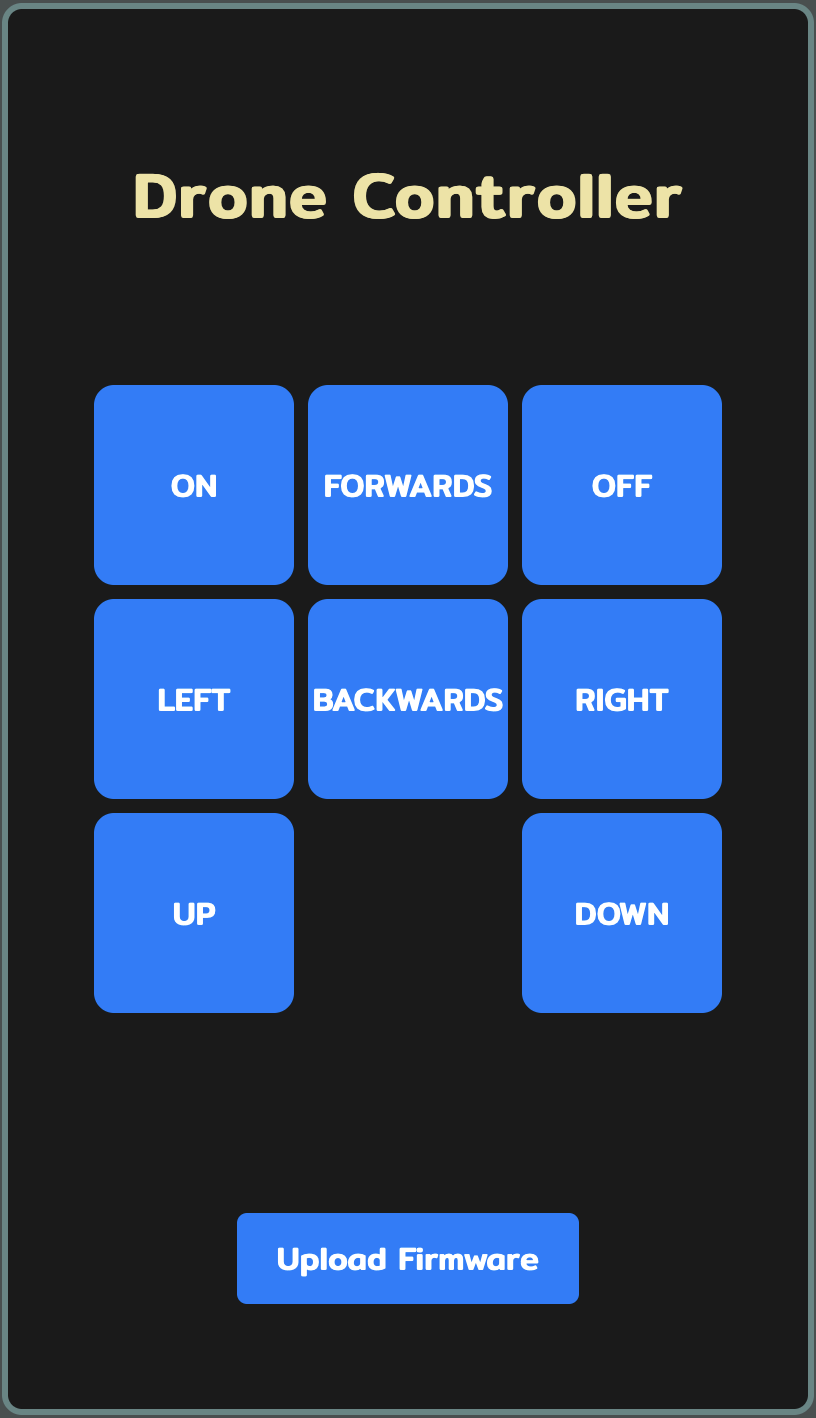
\includegraphics[scale=0.4]{img/gui.png}
        \caption{Webové rozhraní}
    \end{figure}

\newpage
    
\section{Updatování}
    Změnu firmware provádějte pouza na vlastní nebezpečí. Přepsání jakékoliv části základního kódu může způsobit nefunkčnost drona. Pokud jste se rozhodli si kód jakkoliv upravit, můžete ho jednoduše nahrát přes webové rozhraní. Pokud se nacházíte na ovládacím panelu popsaném v předchozí části, zmáčkněte dolní tlačítka "Upload Firmware". Toto vás přesměruje do updatovacího rozharní. Zaškrtněte políčko "Firmware" a vyberte binárku s vaším kódem. Během procesu flashování NEODPOJUJTE dron od baterie.

\section{Skutečné použití}
     I přes veškerou snahu se dron není schopen sám zvednout. Je tomu tak z důvodu příliš vysoké hmotnosti drona, ze kterého motory nemají dostatečný tah pro vzlet. Více než polovina hmotnosti je tvořena samotnou baterií. Dále by bylo dobré zvážit použití jiných vrtulí. Všechny ostatní funkce fungují. Jediné co by na dronu s nižší hmotností bylo potřeba doladit jsou konstanty u vyvažování pomocí gyroskopu a základní rychlost motorů, kterou se otáčejí bez zadaných příkazů.

\chapter{Verze 2.0}
V závěrečné kapitole navrhuji teoreticky vhodnější a funkční řešení tohoto projektu a popisuji změny, které provádím na hardwaru drona.

\section{PCB}
    U první verze tištěného spoje jsem neměl zkušenost s potřebnou velikosti samotné desky. V nové verzi jsou komponenty navzájem značně přiblíženy. Tím snížíme hmotnost drona o několik gramů a nebudeme plýtvat materiálem zbytečným volným místem na desce. Dále jsem opravil chybu, kde ESP pin EN nebyl na tištěném spoji připojen na 3,3V. Na samotném PCB jsem vyměnil jeden z regulátorů za Step-Down converter. Poslední úpravou je přidání přepínače před baterii, aby se dron mohl vypnout i jiným způsobem, než-li odpojením baterie.

\section{Baterie}
    Po testování drona na plný výkon jsem se rozhodl, že kapacita 780mAh má nevýhodný poměr vůči hmotnosti a pro druhou verzi drona jsem se rozhodl zvolit baterii o skoro poloviční kapacitě pro snížení hmotnosti ze 44g na 18g. Dron sice nebude schopen létat zdaleka tak dlouho, ale bude létat. Tato změna vyžaduje ještě jednu úpravu na PCB a to výměnu JST-XH 2pin za 3pin.

\section{Vrtule}
    Pro teoretické zlepšení tahu vyměním vrtule, za doporučené přímo na stránkách motoru\cite{motorv1} a to za trojlisté 48mm vrtule Micro Whoop. Je možné, že tento krok je zbytečný, ale z důvodu intenzivnějšího proudění vzduchu ho zvolím.

\chapter{Závěr}
Tento projekt měl za cíl najít levnější a dostupnější řešení drona pro lidi, kteří rádi tvoří a raději ušetří tím, že si něco složí sami než-li si koupí předražené sestavené řešení.

Tohoto jsem podle mého názoru dosáhl, protože cena vychází přibližně na 1000 Kč. Samozřejmě pokud někdo nemá například pájecí sadu a musel by si ji pořídit, vyšlo by to na více než cenu běžně dostupných dronů. Toto ale nemůžeme započítat do ceny samotného drona.

Bohužel se mi nepovedlo vytvořit létající verzi drona. Vytvořil jsem funkční kód a návrh řešení.


\newpage

\chapter{Reference}

\makeatletter
\renewcommand{\chapter}{\@gobbletwo}
\makeatother

\printbibliography

\end{document}
